% !TEX TS-program = pdflatex
% !TEX encoding = UTF-8 Unicode

% TeX-M (r1.0)
% For my math classes at UT Austin
% Notes template created by Abdon Morales for the College of Natural Science
% and for the Department of Mathematics and Computer Science
% (c) 2019 - 2024 Abdon Morales and the University of Texas at Austin
% This is a notes template for a LaTeX document using the "article" class for Mathematics (Calculus)
% at the University of Texas at Austin.

% Last change made: Jan 15, 2024 8:41 PM CST

% See "book", "report", "letter" for other types of document.

\documentclass[11pt]{article} % use larger type; default would be 10pt

% Start of Article customization options and addons (for more help and information reference to Overleaf's guides and docs on Latex.
\usepackage[utf8]{inputenc} % set input encoding (not needed with XeLaTeX)

%%% Examples of Article customizations
% These packages are optional, depending whether you want the features they provide.
% See the LaTeX Companion or other references for full information.

%%% PAGE DIMENSIONS
\usepackage{geometry} % to change the page dimensions
\geometry{letterpaper} % or letterpaper (US) or a5paper or....
% \geometry{margin=2in} % for example, change the margins to 2 inches all round
% \geometry{landscape} % set up the page for landscape
%   read geometry.pdf for detailed page layout information

\usepackage{graphicx} % support the \includegraphics command and options

% \usepackage[parfill]{parskip} % Activate to begin paragraphs with an empty line rather than an indent

%%% PACKAGES
\usepackage{booktabs} % for much better looking tables
\usepackage{array} % for better arrays (eg matrices) in maths
\usepackage{paralist} % very flexible & customisable lists (eg. enumerate/itemize, etc.)
\usepackage{verbatim} % adds environment for commenting out blocks of text & for better verbatim
\usepackage{subfig} % make it possible to include more than one captioned figure/table in a single float
\usepackage{exercise}
% Math tools
\usepackage{mathtools}
\usepackage{amsmath}
\usepackage{tikz} % For charts, mathematical graphs, and etc
\usepackage{tcolorbox}
%% Equal symbol for L'Hospital Rule
\newcommand\LR{\stackrel{\mathclap{\normalfont\mbox{L.R}}}{=}}
% These packages are all incorporated in the memoir class to one degree or another...

%%% HEADERS & FOOTERS
\usepackage{fancyhdr} % This should be set AFTER setting up the page geometry
\pagestyle{fancy} % options: empty , plain , fancy
\renewcommand{\headrulewidth}{0pt} % customise the layout...
\lhead{}\chead{}\rhead{}
\lfoot{}\cfoot{\thepage}\rfoot{}

%%% SECTION TITLE APPEARANCE
\usepackage{sectsty}
\allsectionsfont{\sffamily\mdseries\upshape} % (See the fntguide.pdf for font help)
% (This matches ConTeXt defaults)

%%% ToC (table of contents) APPEARANCE
\usepackage[nottoc,notlof,notlot]{tocbibind} % Put the bibliography in the ToC
\usepackage[titles,subfigure]{tocloft} % Alter the style of the Table of Contents
\renewcommand{\cftsecfont}{\rmfamily\mdseries\upshape}
\renewcommand{\cftsecpagefont}{\rmfamily\mdseries\upshape} % No bold!
%%% END Article customizations

%%% The "real" document content comes below...

\title{Growth Theory}
\author{Abdon Morales \\ The University of Texas at Austin \\ ECO 304L: Introduction to Macroeconomics \\ Wayne Geerling}
\date{\today \\ Chapter 12 : Week 6}
%\date{} % Activate to display a given date or no date (if empty),
         % otherwise the current date is printed 

\begin{document}
\maketitle
\section*{Building, roads, mosquito nets, and other capital are not the key to economic growth.}
If we look around the world, it is easy to spot high-income nations and low-income nations. Rich, developed nations have impressive capital, including highways, factories, office buildings, and laboratories. Poor, underdeveloped nations have fewer modern factories and buildings, and their roads and other infrastructure are often in disrepair. Think of North and South Korea, as we saw in the last chapter, where one can literally see the difference from outer space. Clearly, wealth and physical capital go hand in hand, and it is tempting to conclude that physical capital is the \textit{source} of wealth: if poor nations can just acquire more and better tools, they too, can be wealthy.

However, correlation does not prove causation; physical capital does contribute to growth, but it is less important than you might think. Often, physical capital is the result of growth, rather than the cause of it. Institutions, not infrastructure, are the real key to economic vitality; in the last chapter we saw in concrete terms how institutions matter. This chapter now provides the theoretical backbone of growth analysis; we begin with a brief description of how economic theories develop. After that, we consider the evolution of growth theory, starting with the growth model created by the American economist Robert Solow. The Solow model formed the foundation for growth theory beginning in the 1950s. After discussing the theory and implications of the Solow model, we consider New Growth Theory and its implied policy prescriptions.

\begin{tcolorbox}[width=\textwidth,colback={white},title={Big Questions},colbacktitle=yellow,coltitle=blue]
\begin{itemize}
\item How do macroeconomic theories evolve?
\item What is the Solow growth model?
\item How does technology affect growth?
\item Why are institutions the key to economic growth?
\end{itemize}
\end{tcolorbox}
\section*{\textbf{How do macroeconomic theories evolve?}}
This chapter marks our first major step into macroeconomic theory, or modeling. In \textit{Chapter 2}, we discussed the characteristics of good economic models: they are simple, flexible, and useful for making accurate predictions. In this chapter, we present a model of economic growth that simplifies from the real world yet also helps us make powerful predictions about economic growth. The stakes are high: growth theory and policy have significant impacts on human lives. Therefore, it's important to consistently reevaluate growth theory in light of real-world results.
Today, economists agree that economic growth is determined by a combination of resources, technology, and institutions; but this consensus is the result of an evolution in growth theory that started almost 60 years ago with the contributions of economist Robert Solow. Although the theory has changed significantly over the past two decades, Solow's growth model still forms the core of the New Growth Theory.

In many academic disciplines, new theories are fodder for intellectual debates, with no direct effect on human lives; but in economics, theories are put to thes test in the real world, often very soon after they are first articulated. Figure 12.1 illustrates the relationship between economic ideas and real-world events. At the top of the circle, we begin with observations of the real world, which inform a theory as it develops. Once an economic theory is developed, it can be influence the policies used to pursue certain economic goals. These policies affect the daily lives and well-being of real people. Finally, as economists observe the effects of policy in the real world, they continue to revise economic theory.
\begin{center}
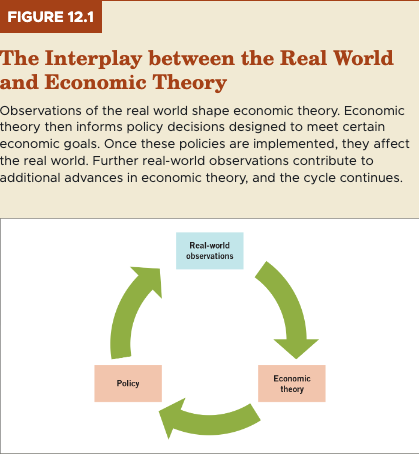
\includegraphics[scale=0.5]{Images/Figure 12.1.png}
\end{center}
Economic growth models affect the the welfare of billions of people worldwide. The result can be beneficial; but if growth theory is wrong or incomplete, it can lead to faulty policy prescriptions that result in poverty. We revisit this point toward the end of the chapter.
\subsection*{The Evolution of Growth Theory}
In 1776, Adam Smith published his renowned book \textit{An Inquiry into the Nature and Causes of the Wealth of Nations}. This book was the first real economics textbook and, as the title indicates, it focused on what makes a nation wealthy. The central question, paraphrased from the title, is: Why do some nations prosper while others do not? More than two centuries later, we still grapple with nature and causes of the wealth of nations.

Economists are not alone in their pursuit of answers to this question. As travel becomes easier and the world economy becomes more integrated, people are more aware of poverty around the globe. Many college students today ask the same questions as economists: Why are so many people poor, and what can be done about it.

This link between economic theory and human welfare is what drives many scholars to study the theory of economic growth. As the Nobel Prize - winning macroeconomist Robert Lucas wrote in 1988: \\
\begin{center}
"Is there some action a government of India could take that would lead the Indian economy to grow like Indonesia's or Egypt's? If so, what exactly? If not, what is it about the 'nature of India' that makes it so? The consequence for human welfare involved in questions like these are simply staggering: \textit{Once one starts to think about them it is hard to think of anything else}."
\end{center}
Economic growth has not always been the primary focus of macroeconomics. After the Great Depression in the 1930s, macroeconomics focused on the study of business cycles, or short-run expansions and contractions. Growth theory began with the Solow model in the 1950s and still serves as the foundation for growth theory, both in method and in policy. Therefore, while growth theory has evolved, it is helpful to consider the Solow model as both a starting point and the basis of current theory.
\section*{\textbf{What is the Solow Growth Model}}
If you travel around the globe and visit nations with different levels of income, you will notice significant differences in physical tools available for use in production. Wealthy nations have more factories, roads, more and better computers - that is, they have more physical capital. Simply viewing the difference in capital, it is easy to conclude that capital automatically yields economic growth.

This was the basic premise of early growth theory: there are rich nations and there are poor nations, and the rich nations are those with capital. Natural resources and human capital are important in the Solow growth model, but the focus is primarily on \textit{physical capital}. So when we speak simply of capital, we mean physical capital; and where human capital is also part of the picture, we will call that labor.

We begin our tour of the Solow model by looking at a nation's production function, which describes how changes in capital affect real output.
\subsection*{A Nation's production function}
The Solow model starts with a \textit{production function} for the entire economy. In macroeconomic theory, a firm's \textbf{production function} describes the relationship between the inputs a firm uses and the output it creates. In equation form, the production function for a single firm is \(q=f(\text{labor, capital}\), where q is the firm's output; this equation says that output \textit{is a function} of the quantities of labor and capital that the firm uses.

In macroeconomics, we extend the production function to an entire nation or economy. The \textbf{aggregate production function} describes the relationship between all the inputs used in the macroeconomy and the economy's total output, where GDP is output. In its simplest form, the aggregate production function tells us that GDP is a function of three broad types of resources, or factors of production, which are inputs used in producing goods and services. These inputs are capital, labor, and natural resources; we can state the aggregate production function in equation form as
\begin{equation}
\text{GDP}= Y = F(\text{labor, capital, natural resources}
\end{equation}
where Y is real output, or GDP.

\subsubsection*{The Focus on capital resources}
While the Solow model recongnizes contributions from both labor and capital, many economists and policymakers focus on capital. As we noted in the chapter opener, early growth theorists saw that capital resources in wealthy nations far exceed those avaliable in developing nations. After all, there are more factories, highways, bridges, and dams in wealthy nations. It seemed logical to conclude that capital is the key to growth.
\begin{center}
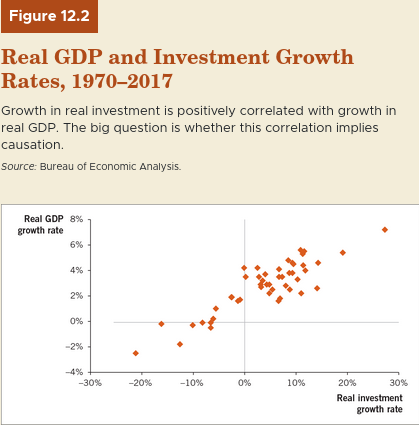
\includegraphics[scale=0.5]{Images/Figure13.2.png}
\end{center}
In addition, periods of investment growth in developed economies are also period of economic expansion. Figure 12.2 plots U.S economic growth rates with investment growth rates from 1970 to 2017. The data show a clear positive correlation between real GDP growth and the rate of investment growth - another reason to believe that investment and capital are the primary sources of economic growth.

Earlier, we noted the interplay of theory and real-world observations; this one example, capital \textit{appears} to cause economic growth because there is such a strong correlation between capital and output. And, certainly, no one disputes that workers are more productive when they have more tools. For now, however, we continue our focus on capital; later, we explore alernative growth sources omitted from this early work.

\subsection*{Diminishing marginal products}
Natural resources also help large, developed macroeconomies, for example, discoveries of natural gas in the United States have increased dramatically over the past two decades. This new energy resource enables the United States to produce more with cheaper resources. To quantify how helpful a resource may be, economists employ the concept of \textit{marginal product}. The \textbf{marginal product} of an input is the change in output assoicated with one additional unit of an input. More resources increase output, so we say the marginal product of each resource is positive.
\subsubsection*{Diminishing marginal product}
Figure 12.3 shows the hypothetical relationship between Chuck's output and the number of ladders he uses. Looking first at the table on the right, not that the second column shows total output (bushels per week), which depends on the number of ladders. The third column shows the marginal product of each ladder; notice that the marginal product declines as more ladders are added. This outcome reflects the principle of \textbf{diminishing marginal product}, which states that the marginal product of an input falls as the quantity of the input rises. Diminishing marginal product generally applies across all factors of production at both microeconomic and macroeconomic level.
\begin{center}
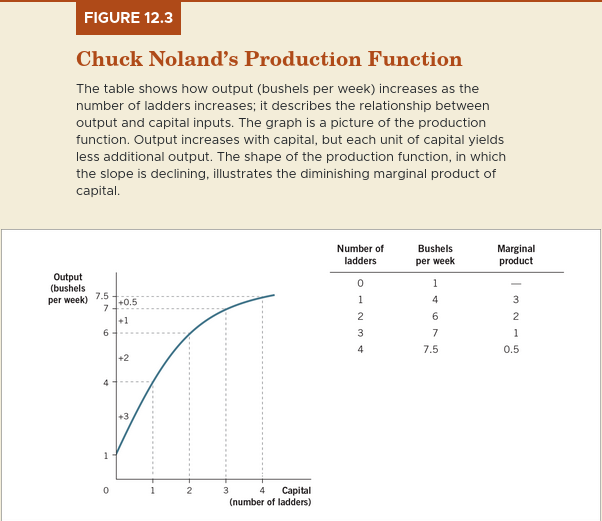
\includegraphics[scale=0.35]{Images/Figure 12.3.png}
\end{center}
The left side of Figure 12.3 is a graph of Chuck's production function: it plots the points from the first two columns of the table on the right. With no ladders, the production function indicates 1 bushel of fruit; but then as ladders are added, output climbs along the curve. The slope of the curve flattens out because the marginal product of the added ladders diminshes.

The principle of diminishing marginal productivity  is not special to our example of one man alone on an island. It is a phenomenon that holds for resources in a macroeconomy in general, and it is a cornerstone insight of the Solow growth model. Sometimes, the name of this principle is simplified to \textit{diminishing returns}; the following discussion places this concept in the macroeconomic context of the U.S interstate highway system.
\subsubsection*{Highways and the production function}
In the United States, we have a system of interstate highways built by the federal government. This interstate highwaay system is essentially a 50,000-mile capital good that we use to help produce GDP. The network of highways connects major cities of the United States; these highways increase GPD in the United States because they help us transport goods and services across the nation.

If the interstate highway system were somehow to close down completetly, GDP would fall immediately; but what would happen to GDP if the government created a second interstate highway system with 50,0000 miles of additional roads crisscrossing the United States? That is, what would be the marginal product of an additional interstate system? The impact would be positive, but much smalller than that of the original network. This interstate exmaple illustrate diminishing returns: the marginal product of highways declines as more and more highways become available.

Figure 12.4 is a graph of the aggergate production function - the production function for the entire economy. On the vertical access, we have outout for the macroeconomy, which is real GDP \(Y\). To simplify, we assume no population growth and so economic growth is represented as movements up along the vertical access. On the horizontal axis, capital resources (K) increases left to right; notice that the slope of the function is positive, which indicates positive marginal product, but the marginal product of capital also declines as more capital is added. For example, the difference in output from the increase in capital from \(K_1\) to \(K_2\) is larger than the change in output from a change in capital from \(K_3\) to \(K_4\). This outcome illustrates the declining marginal product of capital.

The aggregate production function has formed the basis for most discussions in growth theory since 1956. Economic growth is represented by upward movement along the vertical axis; indeed, if ew focus \textit{only} on this simple formulation, economic growth happens only with investment in capital. Diminishing returns, or declining marginal productivity, is the key assumption of the Solow model. As we shall see, this single assumption leads to striking implications for the macroeconomy.
\begin{center}
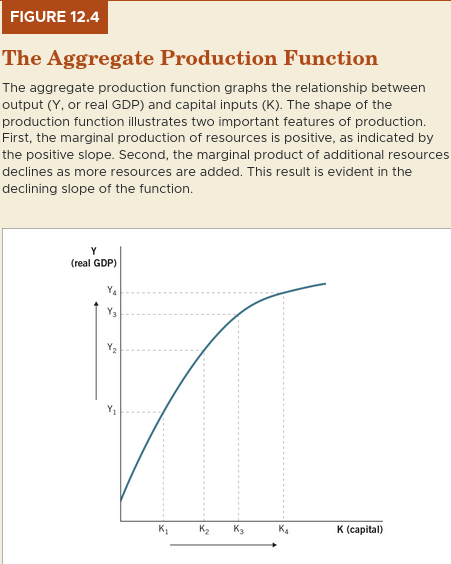
\includegraphics[scale=0.5]{Images/Figure 12.4.png} \end{center}

\subsection*{Implications of the Solow Model}
We can use the basic framework of the production function with an emphasis on capital and diminishing returns to flesh out the two important implications of the Solow model: the conditions of a \textit{steady state} and \textit{convergence}.

\subsubsection*{The steady state}
The Solow model implies the same outcome of large macroeconomies; because the marginal product of capital decreases, at some point there is no reason to build (that is, invest in) more capital. Let's assume this occurs at \(K_3\) in Figure 12.4, this means there is no incentive to build additional capital beyond \(K_3\) because the benefits in terms of additional output no longer exceed the cost of building capital. Since there is no incentive to build capital past \(K_3\), and since we are assuming that capital is the source of growth, the economy stops growing once it reaches \(K_3\).

Once an economy reaches the steady state, there is no change in either capital or real income. The steady state is a direct implication of diminishing returns: when the marginal return to capital declines, at some point there is no incentive to build more capital. The steady state is not a very encouraging situation; you can think of the steady state as the "stagnant state", because when the economy reaches its steady state, real GDP is no longer increasing and economic growth stops.

It is important to distinguish between \textit{investment} and \textit{net investment}; over time, capital wears out: roads get potholes, tractors break down, and factories become obsolete. This is known as capital depreciation; \textbf{Depreciation} is a decline in the value of a resource over time, is natural with capital and it erodes the capital stock. Without new investment, capital declines over time, so some positive investment is needed to offset depreciation, but if investment is exactly enough to replace depreciated items, the capital will not increase - and this means no net investment. \textbf{Net investment} is investment minus depreciation; for the capital stock to increase, net ivnestment must be positive.

This distinction between investment and net investment is important when we consider the steady state. In the steady state, net investment equal zero; there may be positive investment, but this is investment to replace worn-out machines and tools. So when an economy reaches its steady state, the capital stock stays constant.

\subsubsection*{Convergence}
If nations with large stocks of capital reach their steady state and stop growing, nations with less capital can catch up by adding to their capital stock. This means that nations all over the globe could potentially converge to the same level of wealth; \textbf{convergence} is the idea that per capita GDPs across nations equalize as nations approach the steady state. Here is the logic of the Solow model: rich nations are rich because they have more capital, but as these nations approach their steady state, the returns to capital decline and the growth slows. When a nation reaches a steady state, its economic growth stops, but if a nation has not yet reached the steady state, adding capital still leads to growth. Therefore, investment in developing nations should yield relatively greater returns, and this outcome should lead to more capital in developing nations.
\begin{center}
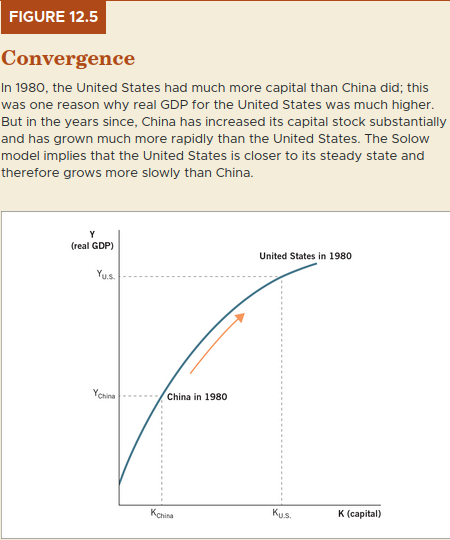
\includegraphics[scale=0.5]{Images/Figure 12.5.png}
\end{center}
Consider the United States and China; in 1980, the United States was wealthy, but China was poor. Figure 12.5 shows both nations as they might have appeared on a production function in 1980. Yet since 1980, growth rates in China have exceeded growth rates in the United States; this blast of growth in China has been accompanied by rapid industrialization - that is, the creation of new capital. According to the Solow model, the new captial in China yields greater returns because the nation started with less capital.

If this basic were completely realistic, new factories in poor nations would typically yield higher return than those in rich nations. Investors seeking to build new factories would turn to nations like Haiti, Nicaragua, and North Korea - nations with relatively small capital stocks.

According to the Solow theory, developing nations should catch up because the older, developed economics have already made new discoveries and have documented mistakes to avoid in the development process. Developing nations can jump right into acquiring the best equipment, tools, and practices.

But reality has been much different from what the theory implies. First, although we have seen cases of rapid growth in poor nations, convergence has been rare; in addition to China, the nations of South Korea, Singapore, India, Chile, and others have done well, but they are exceptions. Very recently, it seems some growth is sprouting in African nations, but for the second half of the twentieth century, most poor nations continued to stagnate, rather than converge to the economic levels of wealthier nations. Second, growth did not seem to slow in wealthy nations over the second half of the twentieth century; recent decades have brought slower growth in many wealth nations, like the United States, but the gap between rich countries and poor countries is widening. More often, countries have shown patterns \textit{divergence} (greater differences between the GDPs of countries) instead of the predicted state of convergence. Given that we have little or no evidence of either a steady state or convergence, economists have reassessed the model, trying to answer the question of why sustained growth continues in wealthy nations. Some economists have pointed to technology as the key driver of this growth, and this is the topic of our next section.

\section*{\textbf{How does technology affect growth}}
Advances in technology, or new ideas, can also lead to economic growth. The Solow model acknowledges technology but does not emphasize how technology develops. In this section, we consider how technological innovations affect the Solow model, and also address assumptions about the way theu occur.

\subsection*{Technology and the production function}
In 1994, Intel introduced a revolutionary computer chip for personal computers - the Pentium chip. The original Pentium could perform 166 million operations per second and was more than three times faster than its predecessor chip (486?); but by 2019, just 25 years later, Intel's new chip, the Core i9 10900X, could perform 1.5 \textit{trillion} operations per second. The new chip costs less and uses less energy than the old chip and yet is about 9,000 times faster!

Thes Intel chips give us a good pictureof what technology does. A computer chip is capital - it is a tool thatt helps us produce. Faster chips means more output with the same amount of capital.

Now let's see how new technology affects the Solow growth model. First, consider the production function; Figure 12.6 shows two production functions: \(F_1\) is the initial production function, when computers are running on Pentium chips. \(F_2\) is the production function after faster chips arrive. Note the new production function is steeper than the old one; the slope is determined by the marginal product of capital, and the new computer chips make capital more productive at all levels. For any given level of capital, real GDP is higher; these are kinds of technological changes that fuel sustained economic growth.
\begin{center}
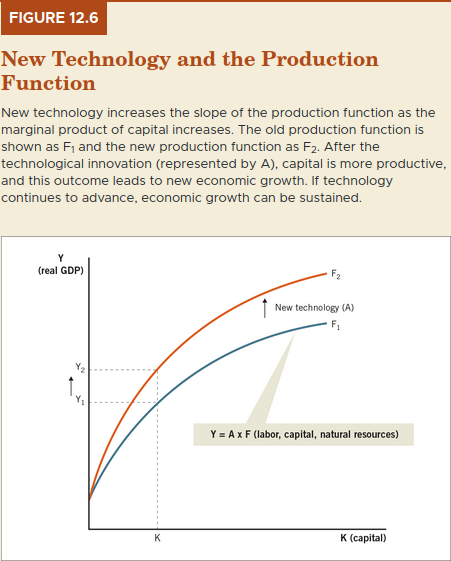
\includegraphics[scale=0.5]{Images/Figure 12.6.png}
\end{center}
We can also use an equation to see how the production function is altered. The aggregate production function now includes an allowance for technological advancement:
\begin{equation}
Y = A \times F (\text{labor, capital, natural resources})
\end{equation}
where A accounts for technological change. The addition of A to the basic model helps explain continued economic growth. Without new technology, the economy eventually reaches a steady state, and growth stops, but new technology means output is higher for any given level of capital, because it makes resources more productive. New technology shifts real output, and therefore income, up to new levels.

Economists and policymakers of course see this shift as very important, and it has driven many political decisions. Before looking at policy implications that derive from the Solow model, let's first look more closely at how technological change occurs in the model.

\subsection*{Exogenous Technological Change}
Why do people innovate? What drives them to create better ways of producing? If technology is the source of sustained growth, the answer to this question is critical.

In the Solow model, there is no real answer to the question of what causes technological innovation. The model assumes that technological change occurs \textit{exogenously}; recall from \underline{Chapter 2} that exogenous factors are the variables outside a model. For our purposes here, the implication is that technological innovations just happen - they are not based on economics. In this sense, technological innovations occur randomly; if technology is exogenous, it is like rainfall: sometimes you get a lot, and sometimes you don't get any. If some nations get more technological innovations than others, that is just thier good fortune.

But if technology is the source of sustained growth, and if technology is exogenous, then economic growth is also exogenous. \textbf{Exogenous growth} is growth that is independent of factors within the economy; when we see innovation occuring in the same places over and over, the Solow model chalks it up to luck. In this view, the innovations are not due to any inherent characteristics of the economies that experience them. Similarly, in this view, poor nations are poor because the random technological innovations happened elsewhere.

If you question the assumption that technological advance is a matter of pure luck, you are not alone. So why did the Solow growth model make this assumption? First, the model assumes that technological progress is tied to scientific advancements, and at times scientific discoveries seem to happen by chance.

Second, this model, like most economic models, is developed mathematically; the assumption of exogenous technological change made the theoretical growth model simpler to solve than an alternative model where technological change is dependent upon multiple factors in the economy.

As we will see in the final section of this chapter, economists in the 1980s developed other models (or techniques) to help incorporate technological change into the original model.

\subsection*{Policy Implications of the Solow Model}
At the beginning of this chapter, we discussed how macroeconomics theory often translates directly into policy. We are now in a position to consider policy prescriptions that emerge from the Solow growth model. Proponents of the Solow model emphasize the importance of capital and technology; thus, for low-income nations to grow, they need the latest technology embedded in capital goods. High-income nations and individuals around the globe can help others grow by providing aid to purchase the latest capital.

As the Solow model grew in the 1950s, two specific types of aid were developed to implement this approach. First, actual capital goods were built with aid from developed nations.

Second, international aid was sent directly to developing nations to help them fund investment in infrastructure such as highways, bridges, and modern ports, as well as other types of capital. These aid payments were intended to help poor nations build capital infrastructure that would pave the way to economic growth.

While there were of course some successes, economists, and policymakers are largely discouraged by the results of these policy initatives.

The application of the Solow model to growth policy was often not successful. In fact, most of the twentieth century witnessed very few success stories and a series of failures. Consider the continent of Africa; thirty-seven African nations achieved independence from 1956 to 1977, offering a unique opporunity to apply the Solow model. Yet by the late twentieth century, it was clear that these policies had failed across the continent, as many African nations were no better off than they were when they gained their independence decades earlier, even while much of the rest of the globe had experienced significant economic gains. Around the end of the twentieth century, these real-world policy results led to a reexamination of growth theory. Economist Dambiasa Moyo wrote a book, \textit{Dead Aid: Why Aid is Not Working and How There Is a Better Way for Africa}, about this failure of international aid across Africa; she argued that foreign aid often led to corruption and nations becoming dependent on this aid, but she also points to policies that can yield growth in low-income nations.

\section*{\textbf{Why are institutions the key to economic growth?}}
Over the past thirty years, a resurgence in growth theory has been spurred by the belief that some economies grow faster \textit{for reasons particular to those economies}. In some nations, and even in pockets within nations, technology advances more quickly than elsewhere; this resurgent growth theory has been dubbed \textbf{New Growth Theory}. It is an approach to long-run growth that focuses on technological change and the incentives fostering innovation inside an economy. The Solow model acknoledges the importance of new ideas and technology, but essentially assumes they spring up exogenously and therefore cannot be predicted. By contrast, New Growth Theory recognizes that economic growth generally appears to be endogenous; \textbf{endogenous growth} is growth driven by factors inside an economy. For example, it is not random coincidence that assembly lines, sewing machines, air conditioning, personal computers, and the Internet were all developed in the United States. These advances spurred economic growth growth and improved people's lives. Why did they all occur in one nation? This is the focus of New Growth Theory.

Economist Paul Romer was awarded the 2018 Nobel Peace Prize in economics in large part based on his work as a founder of New Growth Theory. A famous 1990 paper of his, "Endogenous Technological Change," helped to shift economic theory's focus toward ideas and innovations, and why they occur in some places but no others. Today, many economists stress the importance of institutions as a key factor contributing to endogenous economic growth. We introduced institutions in \underline{Chapter 11}. In the next section, we examine how institutions can provide a foundation for economic growth.
\subsection*{The Role of Institutions}
\begin{center}
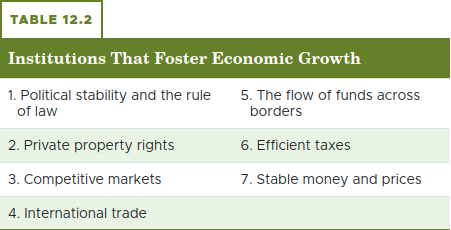
\includegraphics[scale=1]{Images/Table 12.2.png}
\end{center}
Acemoglu and many other economists feel that institutions are a key ingredient in the list of factors driving economic growth. Recall from \textit{Chapter 11} that institutions are significant practices, relationships, or organizations in society that frame the incentives structure within which individuals and business firms act. Institutions are the rules of the game, both formal and informal, framing the environment within which production takes place. They help determine the costs and benefits of production; Table 12.2 lists the institutions important for growth.

If we include institutions in the aggregate production function, we have
\begin{equation}
Y = A \times F\text{labor, capital, natural resources, \textbf{institutions}}
\end{equation}

Insitutions can lay the groundwork for natural endogenous growth; with these institutions in place, there are incentives for new technology to emerge and drive growth.

Figure 12.7 shows how institutions can effect the production function, causing it to rise from \(F_1\) to \(F_2\). Notice that the production function shifts up at all points, since institutions affect output across all levels of capital. Consider the shift toward private property rights that has occurred in China since the 1980s. As we discussed in \underline{Chapter 11}, the shift toward private property rights changed incentives for producers, who now get to keep much of the income from their output. This change created the incentives for the exploding growth we now see in China.

\subsection*{Institutions determine incentives}
We need to consider how institutions affect production decisions; let's begin with an individual firm's decision to produce. Imagine you are considering whether to open a new website design business. You decide you will start such a business only if you expect to at least break even - that is, your payoff must cover your costs. We can state this common condition as follows:
\begin{equation}
\text{Voluntary investment and production occur only if expected payoff} \geq \text{costs.}
\end{equation}

The payoffs come later than the costs and are uncertain, which is why we call them \textit{expected payoffs}.
\begin{center}
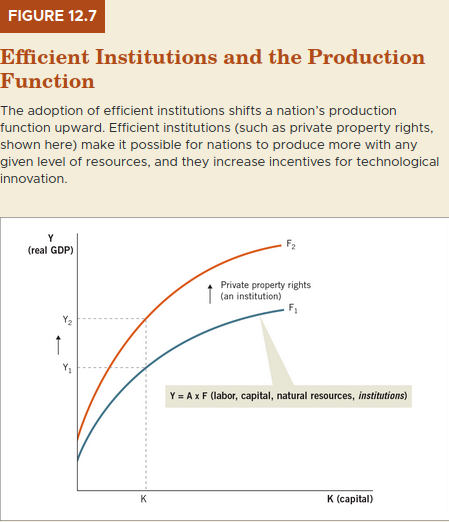
\includegraphics[scale=0.5]{Images/Table 12.7.png}
\end{center}
No matter what your output, the payoffs come after production and after sales. The exact time lag depends on the type of output, but payoffs from output come sometime after expenditures on resources; because of the delay and the resource required, firms need to believe that resource expenditures, including time, patience, and effort, will offer a real payoff in the future.

Or consider your decision to invest in your human capital by attending college: why are you and your family voluntarily spending so much of your resources on the development of your human capital? The answer must be that you expect the return to be greater than the cost. That is, you expect to gain more from your college education than you pay for it; and you probably will, even if it takes a few years to realize the greatest monetary returns.

Investment and production occur naturally if future payoffs are significant and predictable - that is, if the incentives for investment and production are strong enough. These incentives are determined by institutions. Institutions that foster growth are institution that create incentives for technological change; in \textit{Chapter 11}, we saw that the institutions most important for growth include private property rights, political stability and the rule of law, competitive and open markets, the flow of funds across the borders, efficient taxes, and stable money and prices (see Table 12.2). These institutions create incentives for technological innovation and investment in both labor and capital; Figure 12.8 illustrates this relationship between institutions and economic growth. Institutions create incentives for production and investment; if the righ incentives are in place, production and investment occur naturally, and the result is more labor, more capital, and technological advancement - all of which lead to economic growth.

\begin{center}
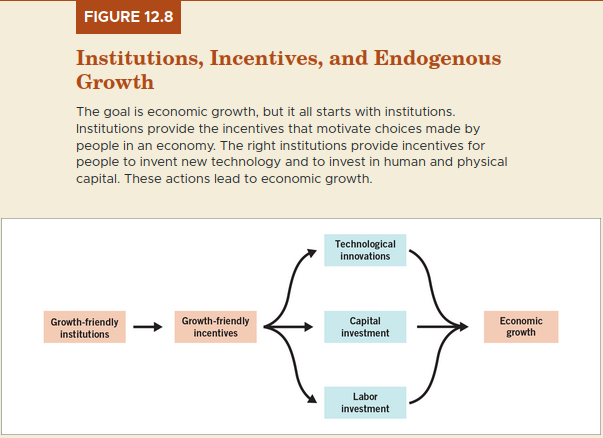
\includegraphics[scale=0.5]{Images/Figure 12.8.png}\\
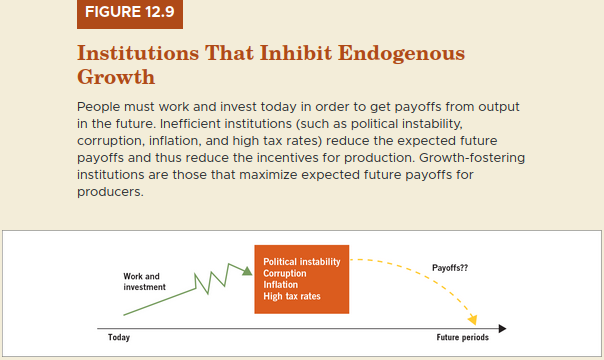
\includegraphics[scale=0.5]{Images/Figure 12.9.png}
\end{center}
As Daron Acemoglu observed in Nogales, weak or malfunctioning institutions can also act to reduce expected payoffs, through corruption, political instability, high and variable inflation, and high tax rates. A key to sustained growth is to eliminate these barriers; Figure 12.9 illustrates how ineffcient institutions impede growth. Because payoffs from productive actions come in the future, anything that reduces the likelihood of these payoffs reduces the incentive for investment today. Resources are not enough; some nations grow faster due to their institutions, others grow slowly because of theirs. Unless institutions are the same across nations we should not expect convergence.

New Growth Theory acknowledges the core truths of the Solow model: resources and technology are resources of economic growth; but it also recognizes the importance of institutions for technological change. This emphasis on institutions matter for policy.

\section*{\textbf{Conclusion}}
We opened this chapter with the misconception that physical capital is the essential ingredient for economic growth. We have seen that while capital is helpful, physical tools are not enough to ensure long-run growth; without institutions that provide incentives to produce, sustained growth does not take root.

Many people think macroeconomics is all about business cycles and recessions; our goal in this chapter has been to present the ideas behind long-run growth theory, rather than short-run cycles. In \underline{Chapter 13}, we present a model that economists use to study short-run business cycles.

\begin{tcolorbox}[width=\textwidth,colback={white},title={Answering the Big Questions},colbacktitle=yellow,coltitle=blue]
\textbf{How do macroeconomic theories evolve?}\\
- Macroeconomics theories evolve in relationship to observations in the real world. Policies often follow from theory; produce results, which in turn influence revisions of economic theory.\\
\textbf{What is the Solow growth model?}\\
- The Solow growth model is a model of economic growth based on a production function for the economy.\\
- The key feature of the production function is diminshing returns. \\
- The Solow growth model posits that diminishing returns lead economies toward a zero-growth steady state.\\
- The Solow growth model further posits that given steady states, economies tend to converge over time.\\
\textbf{How does technology affect growth?} \\
- Technology is a source of sustained economic growth.\\
- In the Solow model, technology is exogenous.\\
\textbf{Why are institutions the key to economic growth?}\\
- New Growth Theory emphasizes that institutions are the key source of economic growth.\\
- Institutions determine incentives for production.\\
- Efficent institutions can lead to endogenous growth.\\
\end{tcolorbox}

\end{document}
